% UMN doctoral dissertation template.
% Created and customized by Shaozhi Nie with LaTeX implementation assistance
% from OpenAI Codex (GPT-5). See CREDITS.md for attribution.
% Replace every bracketed placeholder before submission.
\documentclass[doctoral,12pt]{uofm}

\usepackage{graphicx}
\usepackage{amsmath}
\usepackage{booktabs}
\usepackage{float}
\usepackage[natbibapa]{apacite}
\usepackage[hidelinks]{hyperref}
\graphicspath{{./figures/}}

% Keep the bibliography in the table of contents and use DOI hyperlinks.
\makeatletter
\renewcommand{\bibsection}{%
  \chapter*{\bibname\@mkboth{\MakeUppercase{\bibname}}{\MakeUppercase{\bibname}}}%
  \addcontentsline{toc}{chapter}{\bibname}%
}
\makeatother
% uofm.cls aliases table-list entries to figure-list entries. Restore the
% correct "Table" prefix for List of Tables.
\makeatletter
\renewcommand*\l@table[2]{\@dottedtocline{1}{0em}{4.8em}{\tablename~#1}{#2}}
\makeatother
\AtBeginDocument{%
  \renewcommand{\bibname}{Bibliography}%
  \renewcommand{\refname}{Bibliography}%
  \renewcommand{\doiprefix}{}%
  \urlstyle{same}%
}
\providecommand{\doi}[1]{}
\renewcommand{\doi}[1]{\href{https://doi.org/#1}{\nolinkurl{https://doi.org/#1}}}

% Hyperlinked cross-reference helpers.
\newcommand{\figref}[1]{\hyperref[#1]{Figure~\ref*{#1}}}
\newcommand{\tabref}[1]{\hyperref[#1]{Table~\ref*{#1}}}
\newcommand{\eqnref}[1]{\hyperref[#1]{Equation~\ref*{#1}}}

% The class resets the table counter by chapter but does not retain the chapter
% prefix in its printed form. This keeps the table labels consistent with figures.
\renewcommand\thetable{\thechapter.\arabic{table}}

\title{Dissertation Title in Title Case}
\author{YOUR NAME}
\degree{Doctor of Philosophy}
\advisor{ADVISOR NAME}
\date{August 2026}
\copyrightyear{2026}

\begin{document}
\maketitle
\copyrightpage

\frontmatter
\chapter*{Acknowledgments}
\addcontentsline{toc}{chapter}{Acknowledgments}

I thank my advisor, committee members, collaborators, family, and friends for their guidance and support. Replace this paragraph with your acknowledgments.

\chapter*{Dedication}
\addcontentsline{toc}{chapter}{Dedication}

\begin{center}
For [DEDICATION].
\end{center}

\chapter*{Abstract}
\addcontentsline{toc}{chapter}{Abstract}

This dissertation examines [RESEARCH QUESTION]. The first study [BRIEFLY DESCRIBE METHOD]. The second study [BRIEFLY DESCRIBE METHOD]. Together, the findings show [MAIN CONTRIBUTION]. Replace this text with an abstract that summarizes the motivation, approach, central results, and implications of your dissertation.

\clearpage
\tableofcontents
\clearpage
\listoffigures
\listoftables

\mainmatter
\chapter{Introduction}\label{chap:introduction}

\section{Background and Motivation}

Introduce the broad problem, explain why it matters, and state the gap that motivates the dissertation. Use citations through the \texttt{.bib} file, for example \citep{knuth1984}.

\section{Research Questions}

State the central research question and the specific aims. Each chapter should contribute a distinct part of the overall argument.

\subsection{Example Third-Level Heading}

Use third-level headings only when they improve navigation. Keep the wording parallel across related sections.

\section{Dissertation Roadmap}

Briefly describe what each remaining chapter contributes. For example, Chapter~\ref{chap:methods} presents the methods, and Chapter~\ref{chap:results} presents an example results structure.

\chapter{Methods}\label{chap:methods}

\section{Study Design}

Describe participants, materials, procedures, data sources, and ethics approval as appropriate. Use enough detail for a reader to understand and evaluate the work.

\section{Example Table}

As shown in \tabref{tab:example}, this compact table is a hyperlinked cross-reference. Replace the labels and values with your own data. The table body is set at one-and-a-half spacing to match the dissertation body text.

\begin{table}[H]
  \centering
  \caption{Example study characteristics}
  \label{tab:example}
  \addcontentsline{lot}{table}{\protect\numberline{\thetable.}Example study characteristics}
  \begin{spacing}{1.5}
  \begin{tabular}{lll}
    \toprule
    Group & Sample size & Primary measure \\
    \midrule
    Condition A & 20 & [MEASURE] \\
    Condition B & 20 & [MEASURE] \\
    \bottomrule
  \end{tabular}
  \end{spacing}
\end{table}

\section{Analysis Plan}

Describe preprocessing, statistical analyses, robustness checks, and any deviations from the planned analysis.

\chapter{Theoretical Framework}\label{chap:theory}

\section{Example Displayed Equation}

Define each quantity before using it. An independently displayed equation is automatically numbered and can be cited using \eqnref{eq:example-model}.

\begin{equation}
  y_i = \beta_0 + \beta_1 x_i + \varepsilon_i,
  \label{eq:example-model}
\end{equation}

Here, $y_i$ is the outcome for observation $i$, $x_i$ is a predictor, $\beta_0$ and $\beta_1$ are model parameters, and $\varepsilon_i$ is an error term. Replace this example with the equations used in your dissertation.

\section{Hypotheses}

State the hypotheses or predictions that follow from the framework. Use consistent terminology throughout the document.

\chapter{Results}\label{chap:results}

\section{Example Figure}

Figures should be introduced in the text before they appear. As shown in \figref{fig:example}, Elliott Hall is used here as an example figure that you should replace with a final, accessible research figure.

\begin{figure}[p]
  \centering
  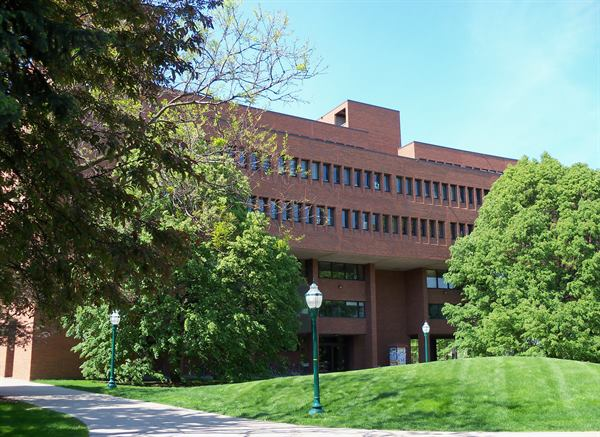
\includegraphics[width=\textwidth,height=0.62\textheight,keepaspectratio]{elliott-hall-cc-by-sa-3.0-template.jpg}
  \caption{Elliott Hall at the Minneapolis campus of the University of Minnesota. Photograph by AlexiusHoratius (2010), licensed CC BY-SA 3.0 via Wikimedia Commons. This image demonstrates a full-page figure layout. Replace it with a final research figure and a self-contained caption that defines all symbols, colors, error bars, and abbreviations needed for interpretation.}
  \label{fig:example}
  \addcontentsline{lof}{figure}{\protect\numberline{\thefigure.}Elliott Hall at the University of Minnesota}
\end{figure}

\section{Interpretation}

Report the result, then explain how it bears on the research question. Distinguish observed results from interpretation.

\chapter{Discussion and Conclusion}\label{chap:discussion}

\section{Summary of Contributions}

Summarize the dissertation's central findings and contributions without repeating every result.

\section{Limitations and Future Directions}

Explain important limitations and identify realistic next steps for future research.

\section{Conclusion}

End with a concise statement of the dissertation's contribution.


\bibliographystyle{apacite}
\bibliography{ref}
\begin{appendix}
\renewcommand\thefigure{\thechapter\arabic{figure}}
\chapter[Appendix A: Supplementary Material]{Supplementary Material}\label{app:supplementary}

Use appendices for supporting material that is necessary for completeness but would interrupt the main narrative. Appendix figures are numbered as Figure~A1, Figure~A2, and so on.

\begin{figure}[H]
  \centering
  \fbox{\rule{0pt}{2.7in}\rule{4.8in}{0pt}}
  \caption{Example supplementary figure. Replace the placeholder with supporting material and a self-contained caption.}
  \label{fig:A1-example}
  \addcontentsline{lof}{figure}{\protect\numberline{\thefigure.}Example supplementary figure}
\end{figure}
\end{appendix}

\end{document}
